\documentclass[a4paper]{article}
%\usepackage{simplemargins}

%\usepackage[square]{natbib}
\usepackage{amsmath}
\usepackage{amsfonts}
\usepackage{amssymb}
\usepackage{graphicx}
\usepackage{times}
\usepackage[margin=1.5in]{geometry}
\usepackage{enumitem}

\begin{document}
\pagenumbering{gobble}

\Large
\begin{center}
  \textbf{Modelling Multilevel Rydberg-Atom Electrometry}\\

  \hspace{10pt}

  % Author names and affiliations
  \large
  Matthew Chilcott$^{\dagger 1}$, Matthew Cloutman$^1$, Susi Otto$^1$, Alex Elliott$^2$, Amita B. Deb$^1$,  Niels Kj{\ae}rgaard$^1$ \\

  \hspace{10pt}

  \small
  $^\dagger$ matthew.chilcott@otago.ac.nz\\
  $^1$ Department of Physics, University of Otago\\
  $^2$ Department of Physics, University of Auckland

\end{center}

\hspace{10pt}

\normalsize

Rydberg atoms are exceptional electric-field sensors: they are
inherently SI-traceable, calibration-free and extremely sensitive~[1],
and they able to sense terahertz-frequency fields, bridging the
elusive ``terahertz gap''~[2]. In experiments, the measurement of the
electric field is mapped to the transmission of a probe beam. This has
been demonstrated repeatedly in the literature, though the
complexities of real atoms are ignored and remain unexplained in most
studies. When varying the polarization of the measured field, these
complexities manifest directly in the observations~[3]. We present a
density-matrix treatment of an atomic Rydberg system, a model which
evolves from the commonly-used 4-level system to a Doppler-averaged
53-state system necessary the explain the polarization-dependent
behaviour.

\vspace{20pt}
\begin{center}
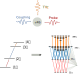
\includegraphics[width=0.7\linewidth]{Figure.pdf}
\end{center}

\vspace{10pt}
\footnotesize

\begin{enumerate}[start=1, label={[\arabic*]}]
\item C. L. Holloway et al., ``Electric field metrology for SI traceability: Systematic measurement uncertainties in electromagnetically induced transparency in atomic vapor''. In: Journal of Applied Physics 121 (2017), p. 233106.      
\item C. G. Wade et al., ``Real-time near-field terahertz imaging with atomic optical fluorescence''. In: Nature Photonics 11 (2017), p. 40-43.
\item J. A. Sedlacek et al., ``Atom-Based Vector Microwave Electrometry Using Rubidium Rydberg Atoms in a Vapor Cell''. In: Physical Review Letters 111 (2013), p. 063001.
\end{enumerate}
\end{document}
